% Point-only paper scaffold copied from Social3_Source_Paper_Brief.pdf.
% Working title: the first candidate title in the brief.
% Reference leads are copied, not bibliographically verified.
\documentclass[11pt,a4paper]{article}
\usepackage[T1]{fontenc}
\usepackage[utf8]{inputenc}
\usepackage[margin=1in]{geometry}
\usepackage{graphicx}
\usepackage[hidelinks]{hyperref}
% Use \socialsource{} for the consistently formatted project name.
\newcommand{\socialsource}{\texorpdfstring{\textit{Social\textsuperscript{3} Source}}{Social3 Source}}
\setlength{\emergencystretch}{3em}
\title{\socialsource{}: Connecting Social Provenance,
Societal Qualities, and Social Purpose on an Open-Source Softwaree Foundation}
\author{Jordi Cabot}
\date{}
\begin{document}
\maketitle
\begin{abstract}
The speed at which software can be created and deployed today has increased dramatically. 
But uwhat is the point of all this software if it does not contribute to society?.
The goal of building any software should be bettering human lives and society. 
And this goes beyond publishing the software as open source; it requires considering how it is developed, the societal qualities it embodies, and the purposes it serves.
This is what I call \socialsource{}. 
This paper presents the concept, principles, and initial discussion for the implementation of \socialsource{}, illustrating how it integrates social considerations into open-source software development.
We have never generated as much software as we do today. 
Let's make sure it is worth it.

\end{abstract}


\section{Introduction}

Creating software is easier than ever thanks to technologies such as low-code development~\cite{Cabot2024LowCode} and, especially, recent advances in artificial intelligence (AI).
These technologies help developers translate ideas into running applications more quickly, improving productivity and reducing the effort required to build software.\footnote{Whether all this software meets appropriate standards of quality is a separate discussion.}
Their significance extends beyond professional developers: they also bring the promise of \emph{citizen development}, in which non-IT professionals create software~\cite{Binzer2022Citizen}, and \emph{end-user development}, in which users adapt and build software for their own needs~\cite{Fischer2004MetaDesign}, closer to everyday practice.
The combination of visual abstractions, reusable components, and natural-language interaction may finally make the longstanding ambition of every citizen becoming a developer of their own applications a practical possibility.

This \emph{development fever}, however, comes at a sustainability cost.
As emphasized by the Karlskrona Manifesto, software sustainability involves interconnected environmental, economic, and social concerns, alongside individual and technical ones~\cite{Becker2015Sustainability}.
Creating, deploying, and operating more applications consumes resources, introduces maintenance and financial commitments, and can reproduce biases or reinforce exclusion.
Lowering the cost of creating an application does not eliminate the costs of sustaining it or the consequences of its use.
We should therefore ensure that the software we create also brings benefits to society, and assess those benefits alongside its costs and potential harms.
Paraphrasing Fei-Fei Li\footnote{\url{https://x.com/drfeifei/status/2102508817653379411}}:
\begin{quote}
The goal of building any software, AI included, should be bettering human lives and society.
\end{quote}

Open-source software grants essential freedoms to inspect, use, modify, and redistribute software~\cite{R3}.
These freedoms enable communities to understand, adapt, share, and maintain the applications on which they depend.
We take open source as a necessary foundation for our proposal, but it is not a sufficient condition to guarantee that software benefits society.
An open licence alone does not establish that development was inclusive, that an application embodies relevant societal qualities, or that its use benefits the people it aims to serve.

To connect these concerns, we introduce \socialsource{}: open-source software that is social in how it is built, in the qualities it embodies, and in the purposes it serves.
The superscript three refers to three complementary social dimensions.
\emph{Social provenance} concerns how and by whom software is developed and governed, including diverse contributions and meaningful participation by affected communities.
\emph{Societal qualities} concern the properties software embodies, such as accessibility, multilingualism, privacy, fairness, affordability, and environmental sustainability.
\emph{Social purpose and impact} concern why software is created or adapted, whom it serves, and the benefits and harms associated with its use, distinguishing intended benefit from observed outcomes.
Together, these dimensions connect development practices, software properties, and societal consequences over an open-source foundation.
We present this concept as an initial position for discussion and a basis for further work on development and assessment.

\begin{center}
\setlength{\fboxsep}{10pt}
\fbox{%
\begin{minipage}{\dimexpr\linewidth-2\fboxsep-2\fboxrule\relax}
\small
\textbf{An illustrative example: an application for migrant services}
\par\medskip
Consider a community organization developing an open-source application to help migrants find local services and navigate administrative procedures.
Its open licence would allow other organizations to inspect, adapt, redistribute, and maintain it.
The scenario illustrates how the three social dimensions of \socialsource{} could be put into practice and assessed.

\medskip
\textbf{Social provenance.}
Migrants, social workers, translators, accessibility specialists, and developers would jointly define requirements, test the application, and influence project decisions.
Documenting their contributions and how their feedback changes the application would provide evidence of meaningful participation beyond code contributions.

\medskip
\textbf{Societal qualities.}
The application would offer appropriate languages, accessible interaction, minimal collection of sensitive information, and support for modest devices and limited connectivity.
Accessibility evaluations, privacy checks, and testing with intended users would help establish whether these qualities are achieved in practice.
Trade-offs would require explicit decisions: for example, AI translation could broaden language coverage while introducing translation errors, resource costs, and reliance on external services.

\medskip
\textbf{Social purpose and impact.}
The application would address service-access barriers identified by the community.
Evaluation would examine whether migrants can find relevant services and complete administrative tasks more easily, while also investigating unintended harms and who remains excluded.
These observations would provide evidence of societal benefit beyond a stated intention to help.

\medskip
Together, these forms of evidence would support an assessment across all three dimensions.
An openly licensed directory developed without migrants, inaccessible to some users, or never adopted by its intended community would leave one or more dimensions unsupported.
The scenario is hypothetical: it illustrates what validation would require, rather than reporting an implemented application or demonstrated impact.
\end{minipage}%
}
\end{center}

The remainder of the paper is structured as follows.
Section~\ref{sec:concept} defines the \socialsource{} concept.
Sections~\ref{sec:provenance}--\ref{sec:purpose} examine its three social dimensions.
Section~\ref{sec:besser} presents a proposed BESSER-based proof of concept, and Section~\ref{sec:related} discusses related concepts and initiatives.
Section~\ref{sec:discussion} examines open challenges and outlines a research agenda, before Section~\ref{sec:conclusion} concludes the paper.

\section{The \socialsource{} concept}
\label{sec:concept}

Figure~\ref{fig:socialsource-foundation} shows the three social dimensions connected through their shared open-source foundation.
\begin{figure}[htbp]
\centering
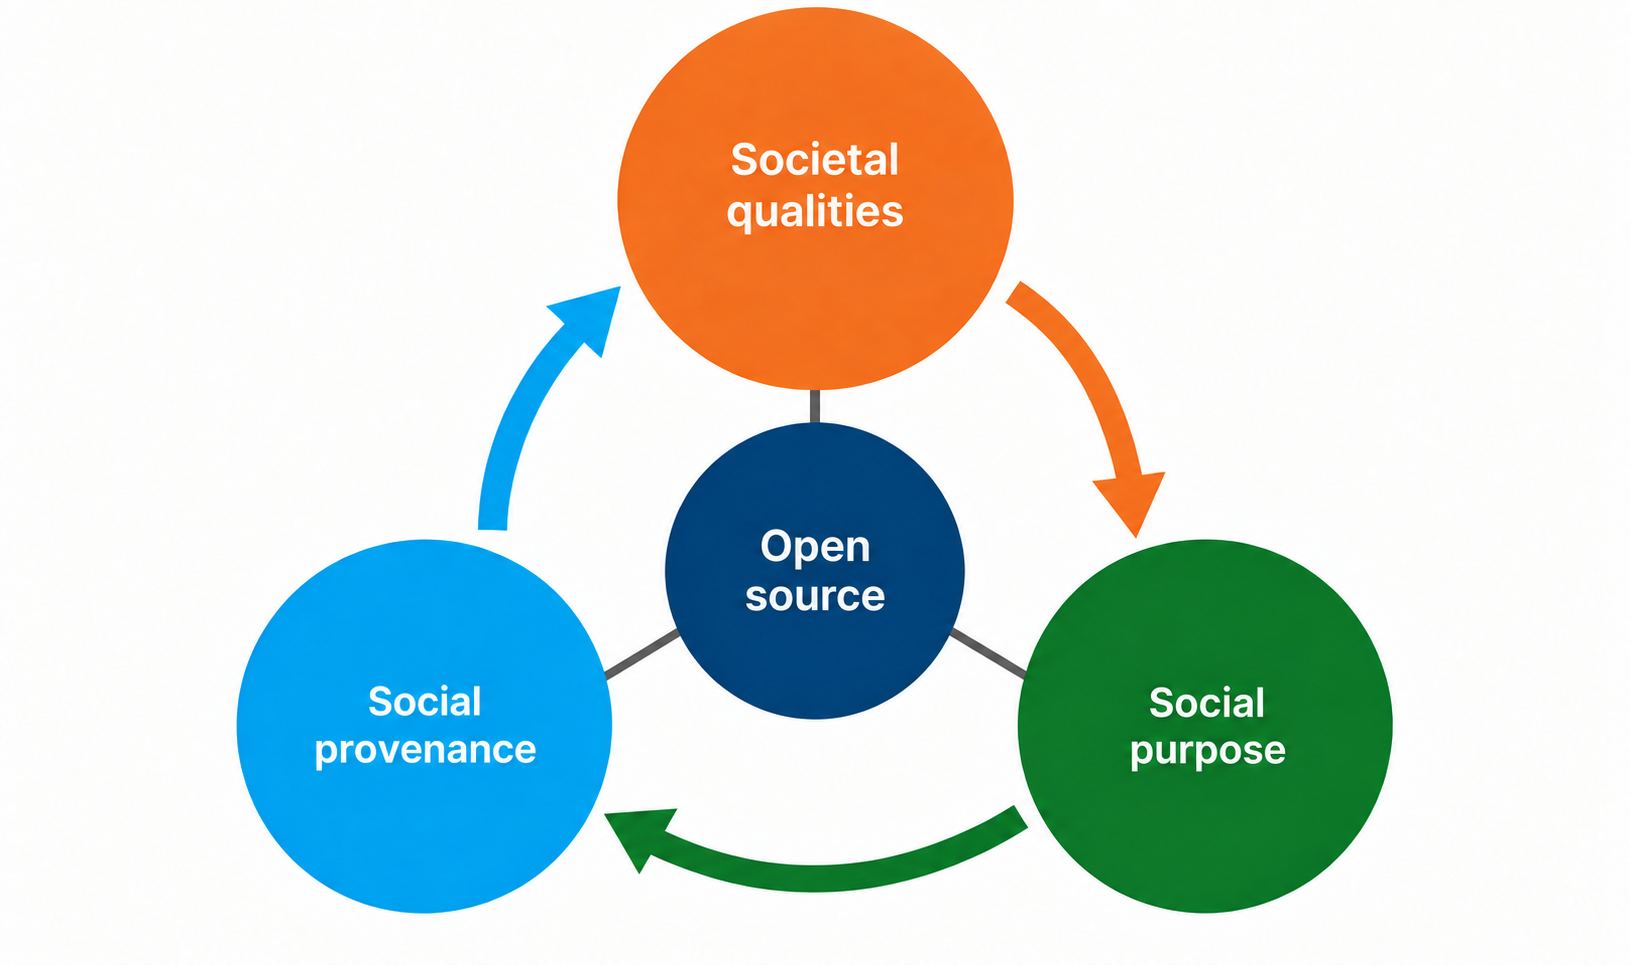
\includegraphics[width=0.9\linewidth]{figures/social3-source-foundation.png}
\caption{The three social dimensions of \socialsource{} share an open-source foundation.
The surrounding arrows emphasize their interdependence across software development, deployment, and evolution.}
\label{fig:socialsource-foundation}
\end{figure}

\begin{itemize}
\item Define the open-source foundation and three dimensions; explain Social\textsuperscript{3}; clarify scope, boundaries, and the distinction between an initial conceptual position and a finished standard.
\end{itemize}

\begin{itemize}
\item Open-source foundation: under what conditions it is shared Use genuinely open-source licensing, with rights to use, study, modify, and redistribute.
An OSI-approved licence is the proposed operational reference \cite{R3}.
Open governance, documentation, standards, and roadmaps can strengthen a project, but they are distinct from its licensing status.
A proprietary project may be socially responsible without meeting this proposal's open-source foundation.
\item The three meanings of social
\item Social provenance: how and by whom.
Diverse, inclusive, transparent, and socially responsible development and governance, including meaningful participation by people with different profiles and by affected communities.
\item Societal qualities: what.
Properties such as accessibility, multilingualism, affordability, privacy, fairness, environmental sustainability, and suitability for users with different resources and circumstances.
\item Social purpose and impact: why, for whom, and with what consequences.
Software created, adapted, or demonstrably used to support communities and public-interest or social missions.
\item ``Societal qualities'' was suggested because it accommodates environmental concerns more naturally than a narrow interpretation of ``social qualities.''
``Social purpose and impact'' distinguishes intended benefit from adoption and observed outcomes; it avoids demanding mature impact evidence from a new project.
\item The superscript \socialsource{}, pronounced ``Social Cubed Source,'' refers to the three social dimensions.
The author proposed this notation to communicate social finality, compliance with social values, and socially diverse development.
It does not denote an exponent in a scoring formula.
A proposed plain-text form is Social3Source.
The name and title have not undergone a separate availability or trademark check.
\item Definitional issues deliberately left open The earlier discussion used a strict classification: all \socialsource{} software is open source, but not all open-source software is \socialsource{}.
Later discussion recognized that the three social dimensions lack qualification thresholds.
Reconcile this by treating openness as mandatory and the dimensions as commitments to be considered and evidenced; leave formal qualification and minimum thresholds to the research agenda.
\item Avoid equating any one of the following with the complete concept: a diverse contributor list, a single accessible feature, an open repository, an NGO customer, or the theoretical possibility that an NGO could use the software.
Also avoid implying that commercial activity is incompatible with social purpose.
\item Possible concise formulation Open by licence, social by process, responsible by design, and purposeful in use.
This is a candidate explanatory phrase, not an additional set of dimensions.
\end{itemize}

\section{Social provenance}
\label{sec:provenance}

% Copied from the agreed paper structure, brief page 3.

\begin{itemize}
\item Explain participation, diversity, transparency, governance, funding, and recognition.
Base the discussion particularly on the Software Diversity Card \cite{R2}.
\end{itemize}

\begin{itemize}
\item The central concern is who shaped the software and how decisions were made.
Include developers, domain experts, designers, translators, documenters, testers, issue reporters, target users, governance participants, and funders.
Git commits alone do not capture these contributions.
\item Use the Software Diversity Card as a main foundation.
Its reported scope includes participants, usage context, and governance \cite{R2,R2a}.
It therefore overlaps more than one proposed \socialsource{} dimension; do not portray the mapping as strictly one-to-one.
Verify its detailed metamodel and empirical findings before quoting statistics.
\item Discuss inclusive contribution routes, fair recognition, transparent decision-making, stakeholder involvement, and responsible working practices.
Diversity should be relevant to the project's context, not reduced to an arbitrary demographic threshold.
Participation should include actual influence: the ability to change requirements, question decisions, and reject unsuitable solutions.
\end{itemize}

\section{Societal qualities}
\label{sec:qualities}

% Copied from the agreed paper structure, brief page 3.

\begin{itemize}
\item Discuss accessibility, multilingualism, affordability, privacy, fairness, sustainability, and their contextual relevance.
Explain why they require explicit requirements and trade-offs.
\end{itemize}

\begin{itemize}
\item Explain what properties the software should exhibit for its intended communities.
Candidate qualities include accessible interaction; appropriate languages and cultural adaptations; affordability and low operational burden; privacy and data minimization; fairness; security; low environmental impact; portability; and operation on modest devices or unreliable networks.
\item The list is illustrative, not an exhaustive universal checklist.
Some qualities will matter differently in different contexts.
The paper should explain how priorities and minimum constraints can be made explicit, while acknowledging that no solution maximizes every objective.
\item Keep separate a stated commitment, a feature implemented in code, a property verified in a running application, and the quality experienced by users.
These are different kinds of evidence.
\end{itemize}

\section{Social purpose and impact}
\label{sec:purpose}

% Copied from the agreed paper structure, brief page 3.

\begin{itemize}
\item Distinguish intended beneficiaries, community participation, adaptation, adoption, outcomes, and harms.
Explain why hypothetical usefulness to NGOs is insufficient.
\end{itemize}

\begin{itemize}
\item Move beyond ``can be used by an NGO.''
Ask whether the software is co-designed with, adapted for, or actually used by a community to advance a social mission or reduce technological, economic, or organizational barriers.
\item Differentiate intent (the need and intended beneficiaries), use (adoption and community involvement), and outcomes (benefits, harms, and distribution of effects).
Community adoption and technical usage metrics do not by themselves prove positive impact.
\item NGOs are an important example, not the entire scope.
Public services, informal communities, cooperatives, and other organizations may also be relevant.
General-purpose software can gain a social role through adaptation and use; the relationship between project-level designation and deployment-specific benefit remains an open question.
\end{itemize}

\section{A BESSER-based proof of concept for \socialsource{} development}
\label{sec:besser}

% Copied from the agreed paper structure, brief page 3.

\begin{itemize}
\item Present the proposed end-to-end framework, with particular attention to modeling builders and software, non-expert participation, deterministic generation of selected qualities, and deployment.
Explicitly separate demonstrated capabilities from envisioned extensions.
\end{itemize}

\begin{itemize}
\item show how a new development can model the builders of the software and the software itself, and generate and deploy the application with BESSER, including participation by team members who are not technical experts.
\end{itemize}

\subsection{Model the people and development process}

\begin{itemize}
\item Represent contributors, community representatives, testers, governance bodies, funding sources, responsibilities, and forms of participation.
Build on Software Diversity Card concepts.
Capture requirements work, validation, translation, and other contributions that may not appear in commit histories.
\end{itemize}

\subsection{Model social requirements and trade-offs}

\begin{itemize}
\item Connect stakeholder needs to target communities, relevant qualities, priorities, minimum thresholds, constraints, and acceptable compromises.
A \socialsource{} requirements DSL is a proposed extension and research direction; do not imply that a complete language is already implemented.
\end{itemize}

\subsection{Collaboratively model the application}

\begin{itemize}
\item Use BESSER models and agentic interaction to express domain concepts, data, behavior, workflows, interfaces, and relevant policies.
The intended benefit is that less-technical members can inspect and influence decisions before implementation.
Confirm which model types and interactions are actually supported by the demonstrated version.
\end{itemize}

\subsection{Generate selected societal qualities by construction}

\begin{itemize}
\item Use deterministic transformations and templates to encode reusable practices.
This is a major argument for the hybrid approach: agentic interaction helps elicit intent; explicit models capture decisions; generators systematically implement the covered patterns.
The next section of this brief explains the limits.
\end{itemize}

\subsection{Validate models and generated applications}

\begin{itemize}
\item Potential checks include accessibility, localization coverage, privacy and security properties, licences and dependencies, resource behavior, and traceability to requirements.
Some checks act on models, others on code or running applications.
Present only implemented checks as prototype results.
\end{itemize}

\subsection{Deploy, evolve, and gather evidence}

\begin{itemize}
\item Illustrate deployment with BESSER and preserve links between stakeholders, requirements, models, generated code, and deployed versions.
Operational measurements and beneficiary feedback could support later assessment.
Runtime usage alone cannot establish social impact.
\end{itemize}

\subsection{Produce \socialsource{} documentation}

\begin{itemize}
\item A proposed \socialsource{} Card could summarize open-source status, provenance, requirements, qualities, intended purpose, evidence, limitations, and assessment results.
Human-readable and machine-readable forms would support communication and automation.
This is an extension idea, not a confirmed deliverable.
\end{itemize}

\subsection{State the implementation boundary}

\begin{itemize}
\item Separate existing capabilities, extensions actually built for this work, and future components.
If implementation is limited, describe a proposed framework illustrated by a prototype.
A successful demonstration supports feasibility, not proof that development was inclusive or that positive social impact occurred.
\end{itemize}

\subsection{Societal qualities by construction}

\begin{itemize}
\item The author's key addition Even if not yet implemented, deterministic BESSER generators could already embed good practices so that the applications they generate are, for example, accessible by default.
The paper should make this forward-looking point prominent without converting it into a claim about current BESSER guarantees.
\item Agentic interaction broadens participation; models make social requirements explicit; deterministic generators can systematically implement selected societal practices.
\item Examples of practices generators could encode
\item Accessibility: suitable semantic components, labels, focus behavior, keyboard interaction, and accessible default styling.
Application content and composed interactions still require evaluation.
\item Multilingualism: externalized text, locale-aware formatting, translation resources, and language selection.
Infrastructure does not guarantee accurate or culturally appropriate translations.
\item Privacy and security: privacy-conscious defaults, minimal data collection patterns, appropriate access controls, and secure configuration.
Context-specific requirements remain necessary.
\item Resource use: resource-conscious implementation patterns and deployment options.
Actual energy behavior depends on workload, hosting, dependencies, and use; it must be measured or clearly estimated.
\item Access and autonomy: responsive interfaces, support for modest devices where feasible, open standards, portability, and maintainable generated artifacts.
\item What deterministic generation can and cannot guarantee Determinism means repeatable generation from the same relevant inputs; it does not by itself mean correctness.
A defective generator can reproduce the same defect everywhere.
Claims of qualities ``by construction'' must specify the property, transformation assumptions, validation, and boundaries of the generated artifact.
\item Distinguish good defaults, systematically implemented patterns, tested properties, and formally established guarantees.
Do not claim that whole-application accessibility, fairness, or sustainability follows from using templates.
Custom code, AI-generated additions, content, third-party components, and later modifications can invalidate assumptions.
\item Connection to maintenance and evolution Improving a generator could propagate better practices across regenerated applications.
This is a prospective benefit to explore, alongside versioning, migration, regression testing, and traceability.
Defaults must remain assessable when software evolves.
\item Role in the position paper The broader position is that societal qualities should be considered during construction, rather than only documented or assessed after development.
Keep the technical ambition proportional to a discussion-oriented paper: examples and a scoped prototype are sufficient; universal guarantees are not required.
\end{itemize}

\section{Related concepts and initiatives}
\label{sec:related}

% Copied from the agreed paper structure, brief page 3.

\begin{itemize}
\item Compare existing uses of Social Source, open-source governance, participatory design, responsible and sustainable software, civic technology, humanitarian OSS, Digital Public Goods, and relevant development technologies.
\end{itemize}

\begin{itemize}
\item Defensible novelty claim The proposed contribution is the synthesis of provenance, societal qualities, and social purpose over an open-source foundation, plus its implications for development and assessment.
Do not claim that the constituent values are new, that all earlier work addresses only one dimension, or that a new label alone constitutes the contribution.
\item Earlier uses of Social Source The earlier conversation identified ``Social Source Software,'' associated with David Geilhufe and a methodology linking open source, collaborative development, and software communities serving NGOs.
It also identified the Social Source Foundation.
These are prior-art leads \cite{R7,R8}, to be checked in the original sources before writing historical claims.
The superscript does not remove the obligation to acknowledge prior use.
\item Related-work streams to compare
\item Open source and governance: licensing freedoms, community health, inclusion, contribution practices, and CHAOSS metrics \cite{R3,R5}.
\item Provenance and diversity: Software Diversity Card, stakeholder involvement, and participatory/community-based design \cite{R2}.
\item Product qualities: responsible and sustainable software engineering, values-based design, accessibility, internationalization, privacy, fairness, and sustainability design \cite{R6}.
\item Social purpose: civic technology, humanitarian FOSS, software for social good, public-interest technology, and Digital Public Goods \cite{R4}.
\item Enabling development: agentic interfaces, low-code and model-driven engineering, and deterministic generation \cite{R1,R9}.
\item Digital Public Goods is a particularly important comparison because it already combines openness, social relevance, and safeguards.
Earlier source checking found its standard focused on the core solution rather than local implementations.
Compare the current standard carefully, using a coverage table with nuanced distinctions rather than unsupported yes/no claims.
\end{itemize}

\section{Discussion, open challenges, and research agenda}
\label{sec:discussion}

% Copied from the agreed paper structure, brief page 3.

\begin{itemize}
\item Pair unresolved issues with research directions.
Foreground the requirements DSL, trade-off negotiation, and automatic/semi-automatic assessment of GitHub projects.
Include evidence limitations, governance, dependencies, and accountability.
\end{itemize}

\subsection{Specifying priorities and trade-offs}

\begin{itemize}
\item Author's explicit research challenge How can users define which social dimensions and qualities are more important to them, given that no perfect solution satisfies every objective simultaneously?
A proposed DSL for \socialsource{} requirements would let stakeholders express these choices.
\item Information the language could capture
\item Relevant communities, stakeholders, needs, and the reasons behind requirements.
\item Dimensions and qualities to address, with context-specific priorities or preferences.
\item Minimum thresholds, mandatory constraints, and acceptable compromises.
\item Dependencies or conflicts among objectives, together with decision rationales.
\item Evidence expected to justify fulfillment, and traceability to models, implementation, deployment, and evaluation.
\item Illustrative requirements, not a proposed syntax For the running example: key service information should be available in selected community languages; essential tasks should be usable with keyboard interaction; access should not require unnecessary sensitive data; operational costs should remain within the organization's means.
Stakeholders could favor locally available translations over external AI translation for sensitive material, depending on their needs and constraints.
\item These statements illustrate the information to represent.
Do not assign invented numerical thresholds, introduce a supposedly standardized grammar, or claim that BESSER currently enforces them.
\item Preferences versus obligations Separate negotiable objectives from hard requirements.
A weighting scheme should not silently allow excellent performance in one dimension to compensate for a critical failure elsewhere.
Whether there are universal minimum conditions, and who establishes them, remains open.
\item Whose priorities count?
Stakeholders may disagree.
A DSL records a decision but does not make that decision legitimate.
Research must address elicitation, representative participation, conflict resolution, consent where relevant, accountability, and revision as circumstances change.
Non-experts should be able to contribute through forms or agentic interfaces without learning textual syntax.
\item Connection to development and assessment Requirements could guide generation, configuration, checks, and evidence collection.
The same declarations could contextualize an assessment profile, showing performance against a community's priorities.
This does not establish a valid overall scoring formula; that remains a separate research problem.
\item Suggested agenda entry Develop human- and machine-readable languages and interaction methods for expressing \socialsource{} requirements, priorities, constraints, stakeholder groups, and acceptable trade-offs; investigate traceability and collective negotiation throughout development and evolution.
\end{itemize}

\subsection{Measuring a project's \socialsource{} profile}

\begin{itemize}
\item Author's explicit research challenge How should a project's ``\socialsource{} score'' be measured?
No formula has been chosen.
The desired direction is automatic or semi-automatic evaluation of a GitHub project, including documentation analysis to understand how it was developed and code/application analysis to assess qualities such as accessibility and sustainability.
\item Evidence for each dimension
\item Provenance: project documentation, contribution histories, governance files, funding declarations, issues, discussions, decision records, testing reports, and evidence of community involvement.
\item Societal qualities: models, source code, dependencies, configuration, localization resources, accessibility checks, privacy and security checks, and workload-based resource measurements or explicitly labeled estimates.
\item Purpose and impact: stated beneficiaries, deployments, partnerships, adoption reports, community feedback, documented outcomes, and reports of unintended harm.
Much of this may live outside GitHub.
\item Working assessment design, not an agreed formula A suggested starting point is an open-source eligibility gate plus separate profiles for the three dimensions, accompanied by evidence completeness and confidence.
An aggregate score could later be investigated, possibly contextualized by DSL-defined priorities.
Do not present this architecture as a validated metric or settled author decision.
\item Questions include indicator selection, normalization, weighting, aggregation, uncertainty, comparability, and safeguards against compensating for critical failures.
A single number may be convenient but can conceal important differences between projects.
\item Evidence and inference must remain distinguishable Distinguish declared claims, documentary evidence, independently checked properties, and observed outcomes.
These are proposed evidence categories, not a universal ordinal scale.
Missing documentation is not proof of a bad practice.
Public documentation is also not proof that the practice actually occurred.
\item Do not infer sensitive contributor demographics from names, photos, or location guesses.
Document participation through appropriate, voluntarily supplied evidence.
Automated accessibility tools cover only some issues; code inspection cannot establish actual energy consumption or lived user experience; adoption does not prove beneficial impact.
\item Unit of assessment and change over time Provenance concerns a project and its history; qualities concern a version and configuration; impact concerns a deployment, community, and period.
An assessment should identify these scopes and evidence dates rather than assign a timeless label to a repository.
\item Research validation to propose Future work could evaluate assessors against expert and community review, study disagreement and missing evidence, and test usefulness across contrasting projects.
Candidate designs discussed included 6-10 projects and practitioner interviews; these are optional future studies, not prerequisites or completed work for this arXiv paper.
\end{itemize}

\subsection{Other discussion points and research directions}

\begin{itemize}
\item Keep these within Section~\ref{sec:discussion}.
Pair each issue with the research it motivates rather than separating a list of problems from a second, repetitive research agenda.
\item Qualification, context, and measurement What minimum conditions distinguish \socialsource{} from a general aspiration?
Should the designation be binary, graduated, or a multidimensional profile?
How can assessments remain meaningful across small volunteer projects, mature infrastructure, and community-specific applications?
Investigate proportional evidence requirements and context-sensitive assessment.
\item Representation, power, and privacy Who legitimately represents a community?
How can participation affect decisions rather than become symbolic?
How should diversity and provenance be reported without exposing sensitive personal information?
Investigate participatory methods, privacy-conscious reporting, fair recognition, and transparent governance.
\item Purpose, harms, and attribution Who defines a social mission, and how are conflicting interests considered?
Can inclusive development still produce harmful software?
How can the contribution of software be distinguished from funding, organizational change, or other interventions?
Combine technical evidence with community perspectives and longitudinal study.
\item Dependencies and community autonomy Can a project qualify while relying on proprietary AI APIs, clouds, platforms, or datasets?
Legal openness may coexist with practical dependence.
Study portability, replaceable dependencies, operating costs, access barriers, and the community's ability to maintain or transfer the system.
\item Maintenance and lifecycle accountability How are social requirements preserved as contributors, models, generators, deployments, and communities change?
What happens when funding ends?
Explore ongoing reassessment, versioned cards and requirements, maintenance responsibilities, and sustainable project governance.
\item Avoiding ``social-source washing'' How can attractive claims be distinguished from substantiated practices and outcomes?
Investigate evidence links, independent assessment where appropriate, transparent limitations, and ways to challenge misleading claims.
Certification, procurement criteria, and funding policies are possible later directions, not current commitments.
\item Tool support and empirical usefulness Explore a \socialsource{} Card or metadata model, repository mining, documentation analysis, model/code/runtime checks, and integration with agentic low-code tools.
Case studies with NGOs, civic initiatives, conventional OSS, and Digital Public Goods could test whether the framework reveals useful differences.
\item Threats and limitations to acknowledge The framework embodies normative choices; relevant qualities depend on context; evidence favors well-documented projects; public repositories reveal only part of the process; small or under-resourced communities may face reporting burdens; and social outcomes are difficult to attribute.
The paper's scope is a position and an invitation, not proof that the proposed dimensions are complete.
\end{itemize}

\section{Conclusion}
\label{sec:conclusion}

% Copied from the agreed paper structure, brief page 3.

\begin{itemize}
\item Restate the position and invite debate, refinement, and implementation.
Avoid declaring consensus or claiming validation that has not been performed.
\end{itemize}

\nocite{*}
\bibliographystyle{unsrt}
\bibliography{references}
\end{document}
